\chapter{Results}



\section{Data Analysis}

\subsection{NEM Data}
NEM data was collated for the period from January 2015 to December 2024 for the NSW NEM region. It contains settlement date-time, total demand for the NEM region, and wholesale price per MWh as determined by AEMO. The settlement periods are in 30 minute intervals until the 1st of October 2021, followed by 5 minute settlement periods for the rest of the data.

\subsubsection{Demand}
Figure~\ref{fig:nsw_demand} shows the demand in the NSW NEM over the 10 years with a 30 day rolling average. Figure~\ref{fig:acf_demand_48hr} shows the daily trends of demand whilst Figure~\ref{fig:acf_demand_365d} shows the seasonal variation in demand.

\begin{figure}[H]
    \centering
    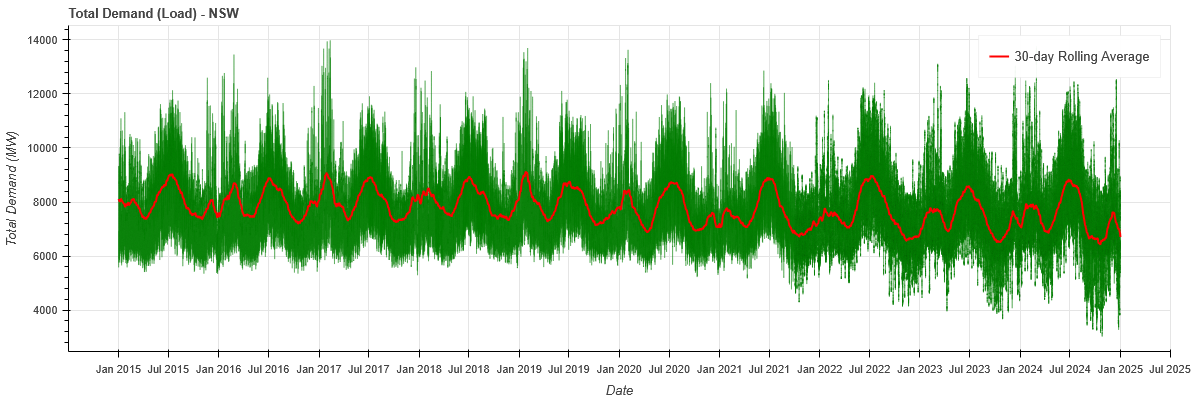
\includegraphics[width=1\textwidth]{images/NSW Demand.png}
    \caption{Demand in NSW NEM with 30 day rolling average}
    \label{fig:nsw_demand}
\end{figure}

\begin{figure}[H]
    \centering
    \begin{subfigure}[b]{\textwidth}
        \centering
        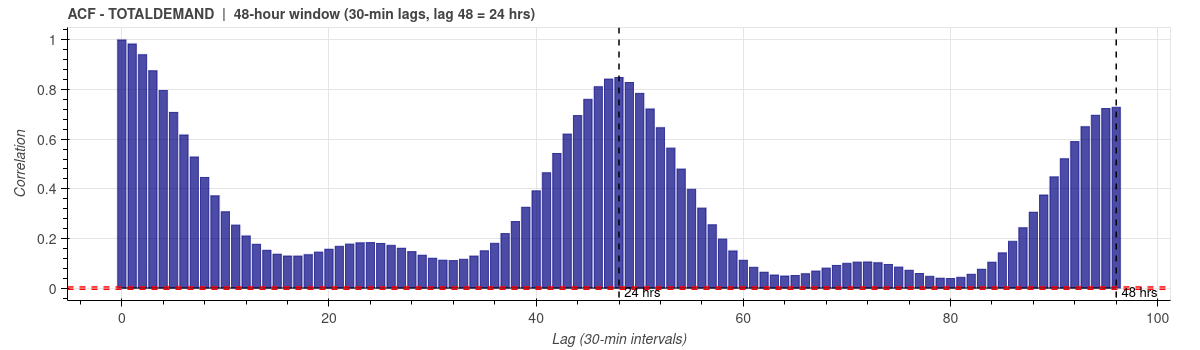
\includegraphics[width=\textwidth]{images/acf_demand.png}
        \caption{ACF - 48 Hours}
        \label{fig:acf_demand_48hr}
    \end{subfigure}
    \\
    \begin{subfigure}[b]{\textwidth}
        \centering
        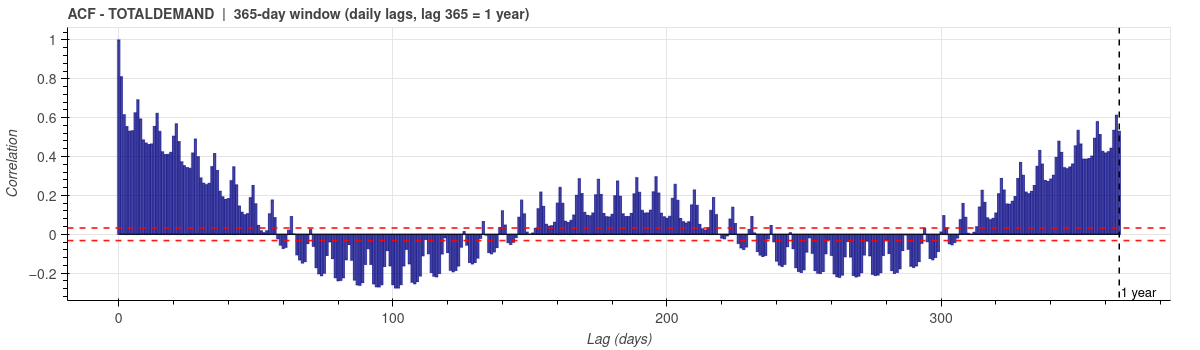
\includegraphics[width=\textwidth]{images/acf_demand_seasonal.png}
        \caption{ACF - 365 Days}
        \label{fig:acf_demand_365d}
    \end{subfigure}
    \caption{Autocorrelation analysis of demand in NSW NEM}
    \label{fig:acf_demand}
\end{figure}

\subsubsection{Regional Reference Price}
The data analysis on the regional reference price (RRP) found a less pronounced autocorrelation than on demand. Figure~\ref{fig:nsw_rrp} shows the wholesale price in the NSW NEM with a rolling average. The figure shows an increasing number of price spike events occurring. Figure~\ref{fig:nsw_rrp_normalised} has been normalised to remove the 1st and 99th percentiles. The results do not show the same seasonality as demand. Figure~\ref{fig:acf_pacf_rrp} however indicates that whilst long-term trends are difficult to interpret in price data, there is a strong daily trend shown by the peaks at 24 and 48 hours.

\begin{figure}[H]
    \centering
    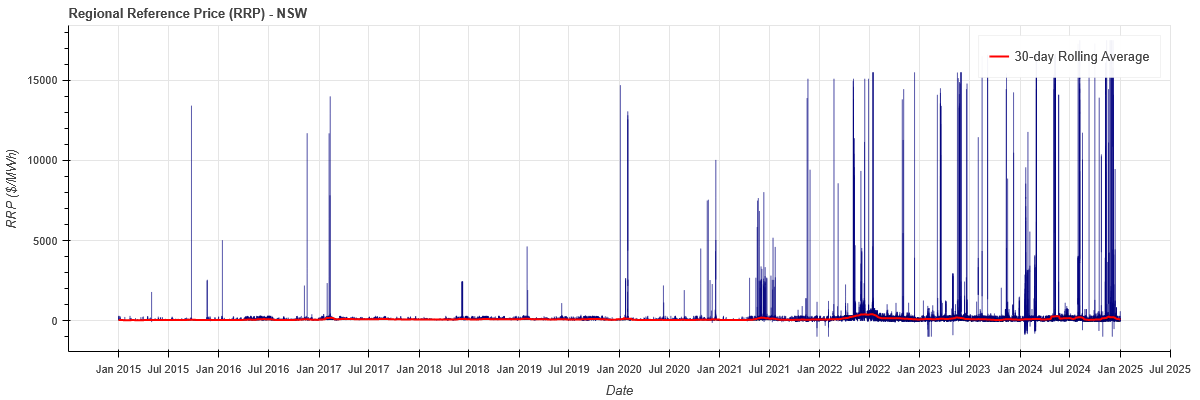
\includegraphics[width=1\textwidth]{images/NSW RRP.png}
    \caption{Wholesale price in NSW NEM with 30 day rolling average}
    \label{fig:nsw_rrp}
\end{figure}



\begin{figure}[H]
    \centering
    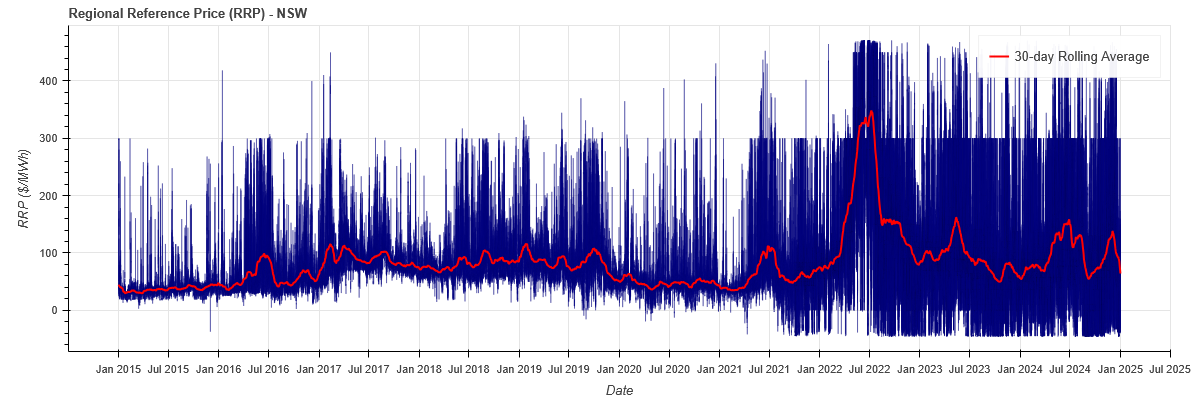
\includegraphics[width=1\textwidth]{images/NSW RRP normalised.png}
    \caption{Wholesale price in NSW NEM with 1st and 99th percentile removed}
    \label{fig:nsw_rrp_normalised}
\end{figure}

\begin{figure}[H]
    \centering
    \begin{subfigure}[b]{\textwidth}
        \centering
        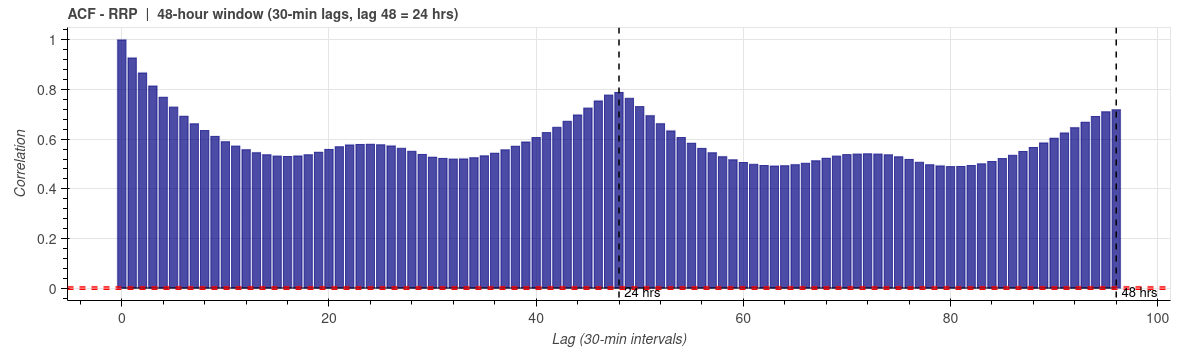
\includegraphics[width=\textwidth]{images/acf_rrp.png}
        \caption{ACF}
        \label{fig:acf_rrp}
    \end{subfigure}
    \\
    \begin{subfigure}[b]{\textwidth}
        \centering
        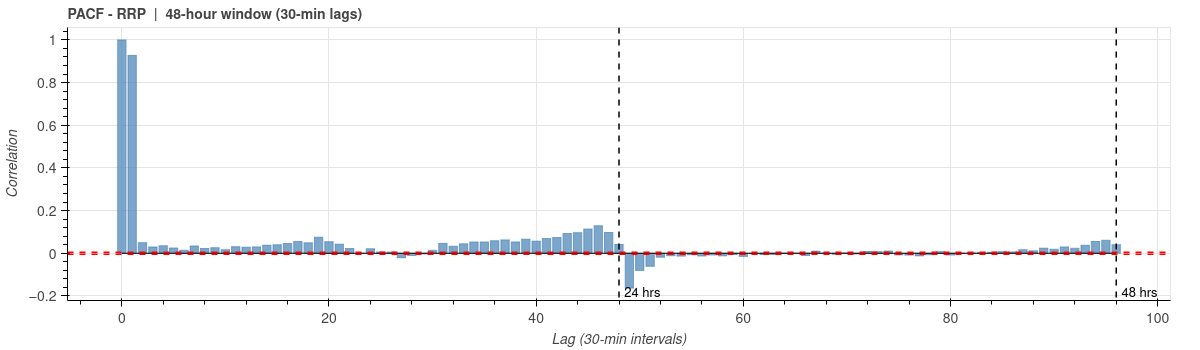
\includegraphics[width=\textwidth]{images/pacf_rrp.png}
        \caption{PACF}
        \label{fig:pacf_rrp}
    \end{subfigure}
    \caption{Autocorrelation analysis of normalised NSW NEM price series}
    \label{fig:acf_pacf_rrp}
\end{figure}

\section{Trading}
To validate the basic operation of a Python framework that consumed NEM and household data, orchestrated battery charge/discharge and produced results for household cost, a basic state machine was designed as shown in Figure~\ref{fig:state_machine}.

\begin{figure}[H]
    \centering
    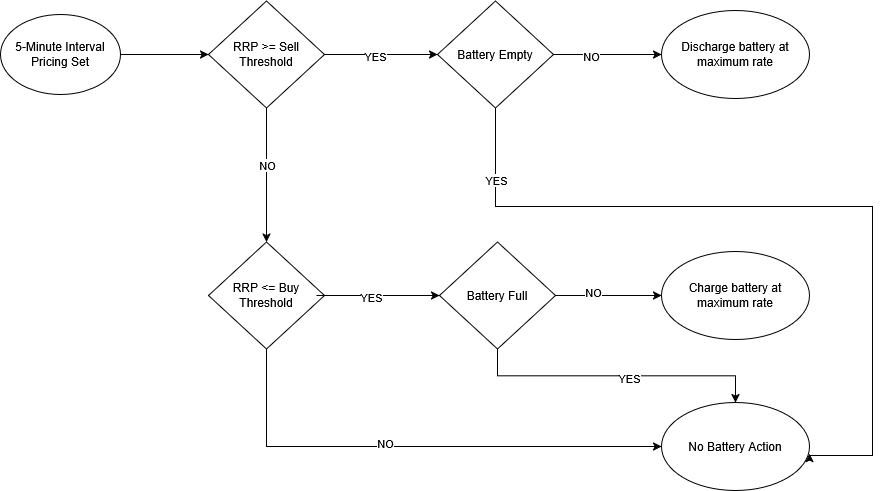
\includegraphics[width=1\textwidth]{images/SimplifiedStateMachineFlowChart.png}
    \caption{A flow chart for state machine trading}
    \label{fig:state_machine}
\end{figure}

The model was trained on a grid search to determine sell thresholds and buy thresholds for a 20 kWh battery with an 11.04 kW inverter. A 60x60 grid search was used with buy ranges from \$0/MWh to \$87.50/MWh and a sell range from \$87.50 to \$189.33. The grid value that produced the lowest net-cost to the consumer was selected. 
The grid was searched using data from December 2024 NEM RRP and household import/export data. The NEM RRP was normalised between the 15th and 85th percentiles for training. The result of the optimisation is summarised in Table~\ref{tab:optimised_thresholds}.

\begin{table}[H]
\centering
\begin{tabular}{lr}
\toprule
\textbf{Parameter} & \textbf{Value} \\
\midrule
Buy threshold  & \$68.22  \\
Sell threshold & \$127.20 \\
Net profit for Dec. 2024     & \$-34.18 \\
\bottomrule
\end{tabular}
\caption{Optimised Thresholds}
\label{tab:optimised_thresholds}
\end{table}

The state machine was then simulated on data from January 2025 with the thresholds in Table~\ref{tab:optimised_thresholds}. The results are summarised in Table~\ref{tab:state_machine_results}. Figure~\ref{fig:statemachine_result} shows the SoC of the battery in relation to RRP and excess solar production. The battery follows a pattern of charging during the day from excess solar and low RRP and discharging in the afternoon.

\begin{table}[h]
\centering
\begin{tabular}{lr}
\toprule
\textbf{Parameter} & \textbf{Value} \\
\midrule
Final Battery State & 18.16 kWh \\
Total Grid Cost     & \$124.18  \\
Total Grid Revenue  & \$179.05  \\
Net Profit          & \$54.88   \\
\bottomrule
\end{tabular}
\caption{State Machine Results January 2025}
\label{tab:state_machine_results}
\end{table}

\begin{figure}[H]
    \centering
    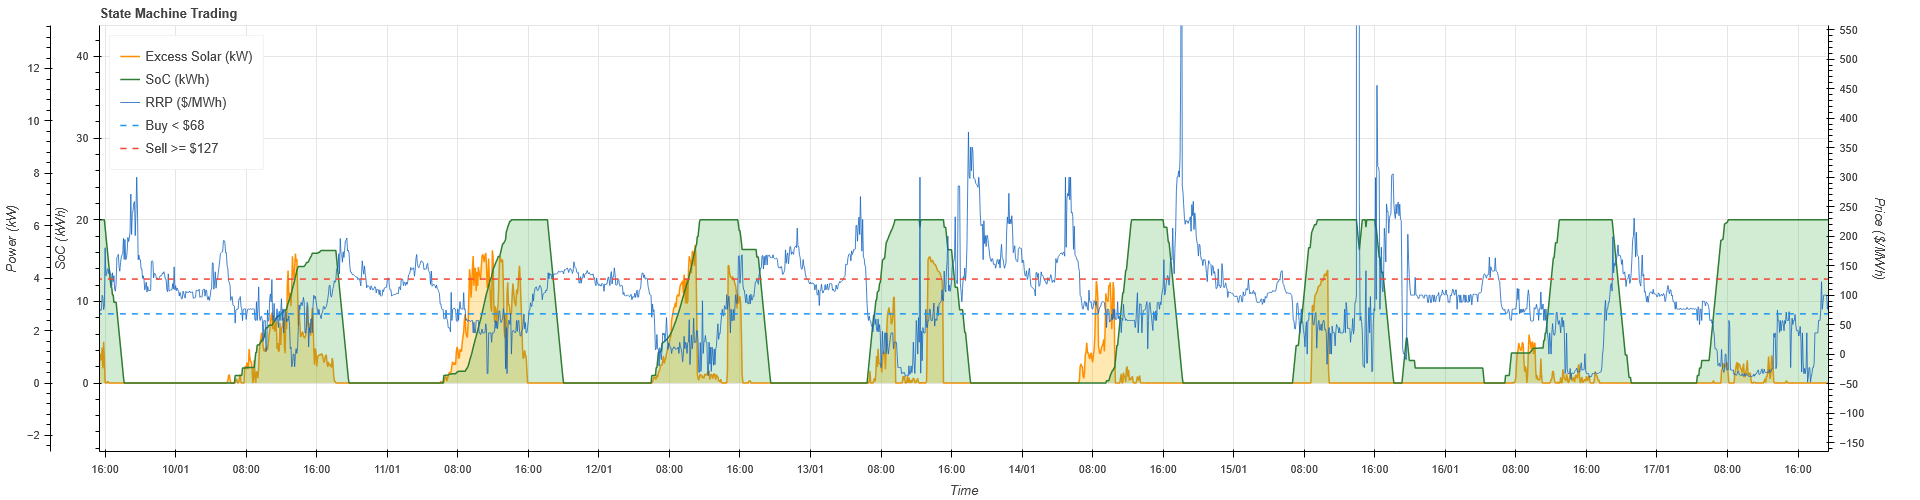
\includegraphics[width=1\textwidth]{images/statemachine_week.png}
    \caption{One week period of state machine control January 2025}
    \label{fig:statemachine_result}
\end{figure}

Figure~\ref{fig:sm_rrp_percentile} provides insight into the pricing events that are contributing most to the export revenue generated. Figure~\ref{fig:sm_rrp_percentile_99-100} shows that exports during price periods in the 99.9th percentile of over \$1510/MWh contribute to 52.5\% of total export revenue over the month. The battery orchestration successfully captured all 9 events where price was in the 99.9th percentile. This distribution of revenue highlights the importance of capturing peak pricing events. It additionally raises questions about how to future-proof a trading system where price peaks become less common as greater commercial BESS capacity is brought online.

\begin{figure}[H]
    \centering
    \begin{subfigure}[b]{0.48\textwidth}
        \centering
        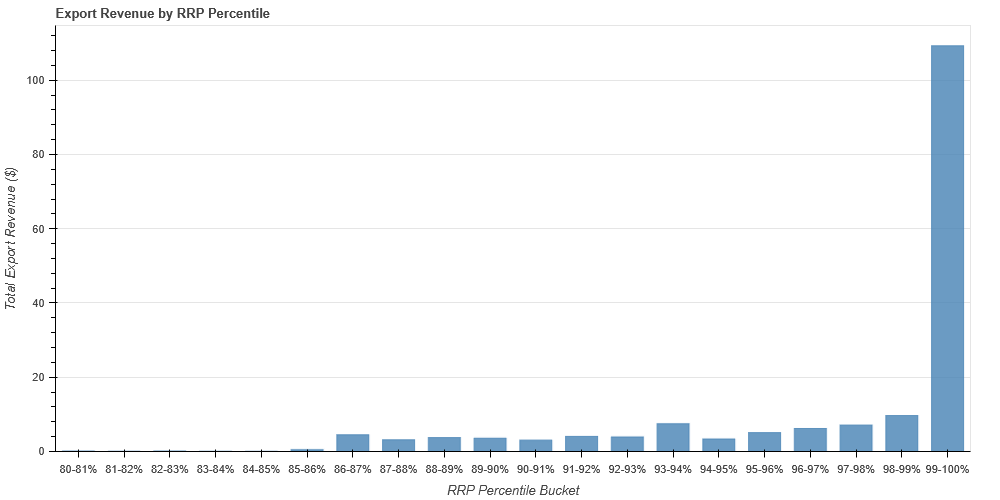
\includegraphics[width=\textwidth]{images/statemachine_rrp_percentile.png}
        \caption{80-100th percentile}
        \label{fig:sm_rrp_percentile_80-100}
    \end{subfigure}
    \hfill
    \begin{subfigure}[b]{0.48\textwidth}
        \centering
        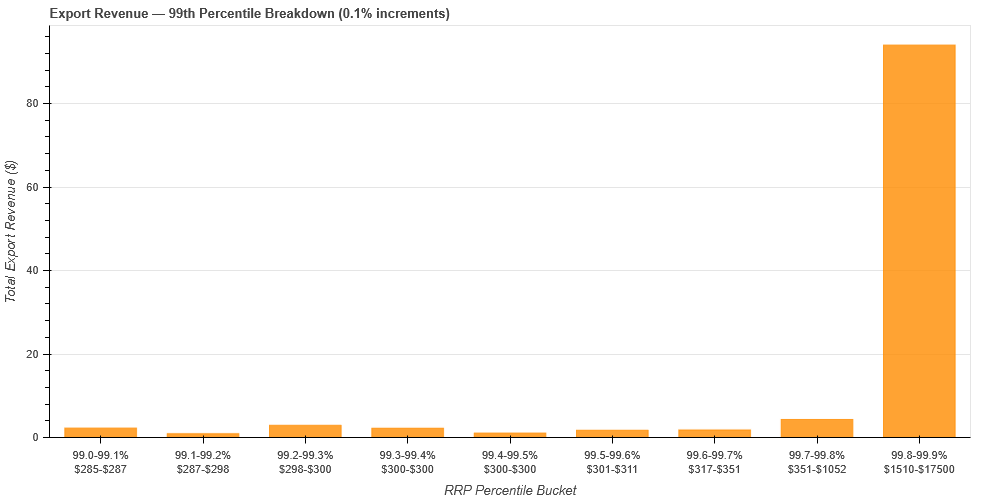
\includegraphics[width=\textwidth]{images/statemachine_rrp_percentile_99_.png}
        \caption{90-99.9th percentile}
        \label{fig:sm_rrp_percentile_99-100}
    \end{subfigure}
    \caption{Export revenue by dispatch period RRP percentile}
    \label{fig:sm_rrp_percentile}
\end{figure}

% -----------------------------------------------------------------------------
% Spot-trading results. Numbers come from code/trading/results/*.csv;
% code/trading/RESULTS.md is the source text.
% -----------------------------------------------------------------------------

\section{Spot trading and retail comparison}
\label{sec:results:trading}

This chapter reports three studies carried out on the battery model of
Chapter~\ref{ch:systemmodel}.
The first solves the mixed-integer linear program (MILP) with perfect foresight to
establish an upper bound and to measure the effect of the cycle-aging cost. The second
replaces perfect foresight with forecasts inside a model predictive control (MPC) loop,
and measures how much of that upper bound a realisable controller recovers. The third
operates the same battery for self-consumption on a set-rate retail tariff, as a
reference for what a household would obtain without market exposure.

\subsection{Common setup}
\label{sec:results:setup}

All results are for the 31 days of January 2025 in the NSW1 region, which is 8928
five-minute dispatch intervals. All monetary values are in Australian dollars for that
month.

The battery is a Tesla Powerwall~3 with $E_{\max} = 13.5$~kWh of usable capacity, a
maximum charge power of 5~kW, a maximum discharge power of 11.04~kW, charge and
discharge efficiencies of $\eta_c = \eta_d = 0.943$, and an initial energy of
$E_0 = 6.75$~kWh. The household is a single dwelling with rooftop solar. Its meter
records net import and net export only, so the model observes the net local power
$G_n - A_n$ and never $G_n$ and $A_n$ separately. Without a battery the household
imports 458~kWh and exports 490~kWh over the month.

Under spot settlement, imported energy is charged at the spot price plus the network
tariff, $R_n + N$ with $N = 10.80$~c/kWh \cite{ausgrid2024networkpricelist},
and exported energy is paid the spot price $R_n$. Battery degradation is represented
inside the MILP by the $J$-segment cycle-aging cost of Xu et al.~\cite{Xu2018}.
Every dispatch schedule is additionally valued after the fact by rainflow cycle counting,
using the stress function $\Phi(\delta) = 5.24\times10^{-4}\,\delta^{2.03}$ and a cell
replacement cost of $R^{\mathrm{cell}} = \$12\,000$. Throughout this chapter, \emph{net
profit} means profit at the meter less the rainflow degradation cost, so that schedules
produced with different values of $J$ are valued on the same basis.

The spot price in January 2025 had a mean of \$83/MWh and a median of \$76/MWh. It was
negative in 15.2\% of intervals, above \$300/MWh in 0.45\% of intervals, and above
\$1000/MWh in ten intervals, which fell on 1, 14, 15 and 22 January. The maximum was the
market price cap of \$17\,500/MWh on 15 January.

\paragraph{No-battery reference.}
On spot settlement the household alone pays \$101.84 for imports and receives \$10.53 for
exports, a net position of $-$\$91.31 for the month. Household results below are the
net position of the whole household, so the value added by the battery is the reported
result minus $-$\$91.31.

% -----------------------------------------------------------------------------
\subsection{Perfect-foresight dispatch and the cost of cycling}
\label{sec:results:milp}

The MILP was solved with a rolling horizon: each window covers 48~hours, the first
24~hours are committed, and the per-segment energy is carried into the next window,
giving 31 windows for the month. Two scenarios were run. In the \emph{household}
scenario the battery sits behind the meter with the solar and load. In the
\emph{battery-only} scenario the household terms are zero and the battery trades alone.
Results are given in Tables~\ref{tab:milp:household} and~\ref{tab:milp:bess}.

\begin{table}[htbp]
    \centering
    \small
    \caption{Perfect-foresight MILP, household scenario, January 2025. Error is the
    relative difference between the degradation cost inside the MILP and the rainflow
    cost. The state machine uses thresholds of \$68.22 and \$127.20 per MWh on a 20~kWh
    lossless battery and is included for qualitative comparison only.}
    \label{tab:milp:household}
    \begin{tabular}{@{}lrrrrrr@{}}
        \toprule
        Model & \shortstack{Profit\\at meter (\$)} & \shortstack{Rainflow\\deg.\ (\$)} &
        \shortstack{Net\\profit (\$)} & \shortstack{Life\\lost (\%)} &
        \shortstack{Full\\cycles} & \shortstack{Error\\(\%)} \\
        \midrule
        $J=1$, $R^{\mathrm{cell}}=0$ & 95.38 & 194.76 & $-99.38$ & 1.623 & 42.3 & -- \\
        $J=1$  & 14.92 & 2.43  & 12.49 & 0.020 & 1.0  & 168 \\
        $J=2$  & 43.97 & 22.58 & 21.40 & 0.188 & 8.0  & 15.6 \\
        $J=4$  & 43.84 & 15.10 & 28.74 & 0.126 & 9.3  & 4.2 \\
        $J=8$  & 47.99 & 16.65 & 31.34 & 0.139 & 12.7 & 1.1 \\
        $J=16$ & 49.01 & 16.62 & 32.39 & 0.139 & 15.0 & 4.1 \\
        \midrule
        State machine & 54.88 & 135.82 & $-80.95$ & 1.132 & 25.5 & -- \\
        \bottomrule
    \end{tabular}
\end{table}

\begin{table}[htbp]
    \centering
    \small
    \caption{Perfect-foresight MILP, battery-only scenario, January 2025.}
    \label{tab:milp:bess}
    \begin{tabular}{@{}lrrrrr@{}}
        \toprule
        Model & \shortstack{Profit\\at meter (\$)} & \shortstack{Rainflow\\deg.\ (\$)} &
        \shortstack{Net\\profit (\$)} & \shortstack{Full\\cycles} & \shortstack{Error\\(\%)} \\
        \midrule
        $J=1$, $R^{\mathrm{cell}}=0$ & 136.23 & 139.31 & $-3.09$ & 25.4 & -- \\
        $J=1$  & 103.98 & 1.68 & 102.30 & 0.9 & 252 \\
        $J=2$  & 105.91 & 2.94 & 102.98 & 1.4 & 51 \\
        $J=4$  & 113.97 & 6.77 & 107.20 & 4.8 & 12.5 \\
        $J=8$  & 113.41 & 5.22 & 108.19 & 5.0 & 6.9 \\
        $J=16$ & 113.55 & 5.16 & 108.39 & 5.4 & 2.6 \\
        \bottomrule
    \end{tabular}
\end{table}

\paragraph{Ignoring degradation removes the value of trading.}
With $R^{\mathrm{cell}} = 0$ the optimiser earns the most at the meter, \$95.38 in the
household scenario and \$136.23 for the battery alone, but it completes 42 and 25
equivalent full cycles in the month and consumes 1.6\% and 1.2\% of the battery's cycle
life. Once that wear is valued by rainflow counting, both scenarios make a net loss. The
threshold state machine fails in the same way: it earns more at the meter than any
degradation-aware MILP and loses all of it to aging, for a net result of $-$\$80.95.

\paragraph{A degradation-aware controller trades about a fifth as often and keeps the profit.}
At $J = 4$ the household battery completes 9.3 equivalent full cycles, loses 0.126\% of
its life, and returns a net profit of \$28.74. Relative to the no-battery position this
is \$120.05 of value added after \$15.10 of aging.

\paragraph{Four segments are sufficient.}
With a single segment, all cycling is priced at one marginal cost and the battery barely
trades. Net profit rises steeply up to $J = 4$ and then flattens: \$28.74, \$31.34 and
\$32.39 at $J = 4$, 8 and 16, for solve times of 13~s, 27~s and 63~s. At $J = 4$ the
degradation cost inside the MILP agrees with the rainflow cost to within 4.2\%. The
error is not monotonic in $J$ beyond this point (1.1\% at $J = 8$ and 4.1\% at
$J = 16$), which indicates that the remaining differences are within the variation of a
single month. $J = 4$ is therefore used for the forecasting study.

\paragraph{Co-located solar and load increase the value of the battery.}
Before aging, the battery adds \$135.16 in the household scenario against \$113.97 when
trading alone. This is consistent with the battery charging from surplus solar that
would otherwise be exported at $R_n$, and discharging into load that would otherwise be
imported at $R_n + N$, so that it earns the network tariff in addition to the price
spread.

% -----------------------------------------------------------------------------
\subsection{Forecast-driven dispatch}
\label{sec:results:mpc}

This study measures the \emph{dispatch value} of a forecast: the net profit obtained
when the MILP plans on that forecast, compared with the net profit under perfect
foresight. The household scenario is used with $J = 4$.

At every five-minute interval the controller solves the MILP over a 24-hour horizon,
implements the first interval only, and repeats, giving 8928 solves per forecaster at
0.14 to 0.33~s each. Following the information structure of
Chapter~\ref{ch:systemmodel}, the price of the current interval is known, because AEMO
publishes it before the interval begins, while all later prices and all net local power,
including that of the current interval, are forecast. The implemented charge and
discharge powers are then settled against the actual price and the actual net local
power. The forecasters are described in Section~\ref{sub:forecast:price}.
The net local power is forecast in every case by the mean of the same five-minute slot
over the previous seven days, which has a mean absolute error of 1.15~kW. The
\emph{perfect price} case uses actual prices with this household forecast, and so
separates the cost of the household forecast from the cost of the price forecast.

\begin{table}[htbp]
    \centering
    \small
    \caption{Forecast accuracy and dispatch value, household scenario, $J=4$, January
    2025. MAE is the mean absolute error of the price forecast over all lead times and
    rMAE is the MAE relative to the seasonal-naive forecast.}
    \label{tab:mpc:headline}
    \begin{tabular}{@{}lrrrrrrr@{}}
        \toprule
        Forecaster & \shortstack{MAE\\(\$/MWh)} & \shortstack{Median\\AE} & rMAE &
        \shortstack{Profit\\at meter (\$)} & \shortstack{Rainflow\\deg.\ (\$)} &
        \shortstack{Net\\profit (\$)} & \shortstack{\% of\\perfect} \\
        \midrule
        Perfect                  & 0     & 0    & --   & 43.85 & 15.11 & 28.74 & 100 \\
        Perfect price            & 0     & 0    & --   & 34.33 & 14.69 & 19.64 & 68 \\
        LSTM                     & 44.6  & 22.0 & 0.73 & 33.29 & 17.35 & 15.94 & 55 \\
        Seasonal naive           & 61.3  & 25.3 & 1.00 & 31.71 & 15.79 & 15.92 & 55 \\
        AEMO pre-dispatch        & 161.6 & 16.4 & 2.63 & 30.24 & 15.57 & 14.67 & 51 \\
        \bottomrule
    \end{tabular}
\end{table}

On the 2024 validation year the LSTM had an MAE of \$70.3/MWh against \$103.1/MWh for
the seasonal-naive forecast, an rMAE of 0.68, with the best model obtained at epoch 5.
January 2025 was not used for training or model selection.

\paragraph{The rolling loop costs nothing under perfect information.}
Perfect foresight on the 24-hour, five-minute MPC loop reproduces the result of the
48-hour rolling solve exactly (\$28.74). Every gap in Table~\ref{tab:mpc:headline} is
therefore caused by forecast error and not by the horizon or the re-planning frequency.

\paragraph{Most of the loss comes from the household forecast, not the price forecast.}
Knowing every price but forecasting the net local power loses \$9.10 of the
\$12.80 to \$14.07 total gap. Measured against the perfect-price case, the price
forecasts cost \$3.70 for the LSTM, \$3.72 for the seasonal-naive forecast and \$4.97
for AEMO pre-dispatch.

\paragraph{A more accurate price forecast did not produce more dispatch value.}
The LSTM reduces the MAE by 27\% relative to the seasonal-naive forecast, from
\$61.3/MWh to \$44.6/MWh, and finishes two cents ahead of it. It earns \$1.59 more at
the meter, but its schedule has deeper cycles (a mean depth of 0.196 against 0.158) and
incurs \$1.56 more in aging.

\begin{table}[htbp]
    \centering
    \small
    \caption{Value added by the battery over the no-battery household, before aging,
    by the spot price of the interval in which it was earned (\$).}
    \label{tab:mpc:bands}
    \begin{tabular}{@{}lrrrrrr@{}}
        \toprule
        $R_n$ (\$/MWh) & Intervals & Perfect & \shortstack{Perfect\\price} & Naive & AEMO & LSTM \\
        \midrule
        $< 0$       & 1411 & 2.35   & $-0.49$ & 0.15   & $-0.25$ & $-0.07$ \\
        0 -- 50     & 1211 & $-1.20$ & $-3.14$ & $-3.04$ & $-3.02$ & $-3.18$ \\
        50 -- 100   & 3928 & 2.02   & 1.40   & 1.44   & 1.37   & 0.79 \\
        100 -- 300  & 2338 & 23.89  & 20.69  & 17.22  & 18.65  & 19.87 \\
        300 -- 1000 & 30   & 6.57   & 5.65   & 5.71   & 4.24   & 5.66 \\
        $> 1000$    & 10   & 101.53 & 101.53 & 101.53 & 100.56 & 101.53 \\
        \midrule
        Total       & 8928 & 135.16 & 125.64 & 123.01 & 121.55 & 124.60 \\
        \bottomrule
    \end{tabular}
\end{table}

\paragraph{Three quarters of the value is earned in ten intervals, and every controller captures it.}
Table~\ref{tab:mpc:bands} separates the value added by price band. Of the \$135.16 added
under perfect foresight, \$101.53 is earned in the 50 minutes during which the price
exceeded \$1000/MWh. All five controllers discharge at the full 11.04~kW in those
intervals, with the single exception of the AEMO-driven controller in the
\$1052/MWh interval on 14 January, at a cost of \$0.97. This occurs because the price of
the current interval is observed before dispatch, and because each controller happened
to be holding charge when each spike arrived. None of the forecasters predicted these
spikes, and none needed to. The differences between forecasters arise instead in
ordinary arbitrage: in the \$100 to \$300/MWh band, where perfect foresight earns
\$23.89 against \$17.22 to \$20.69, and at negative prices, where it earns \$2.35
against approximately zero.

\paragraph{AEMO pre-dispatch is the most accurate forecast in normal conditions and the least accurate on average.}
It has the lowest median error (\$16.4/MWh) and the highest MAE (\$161.6/MWh). It
forecast prices near the market price cap on the hot days of 14--15 and 21--22 January
that largely did not eventuate: 1.0\% of its forecast values exceed \$1000/MWh, against
0.1\% of actual prices. With forecast errors clipped at \$1000/MWh its MAE is
\$48.9/MWh, between the LSTM (\$44.7/MWh) and the seasonal-naive forecast
(\$53.2/MWh). In dispatch it finishes \$1.25 below the seasonal-naive forecast.

\paragraph{Forecast accuracy and dispatch value are only loosely related.}
Ranked by MAE the order is LSTM, seasonal naive, AEMO pre-dispatch. Ranked by net
profit the LSTM and the seasonal-naive forecast are level and AEMO pre-dispatch is
slightly behind, with all three within \$1.27 of one another.

\subsubsection{Implications}
\label{sec:results:mpc:implications}

The assumption that carries the most weight in this study is that the price of the
current interval is known before the dispatch decision is made. It is what secures the
\$101.53 earned during price spikes. The assumption is realistic, but its value has not
yet been measured, and doing so requires only that the study be repeated with the
current-interval price forecast rather than observed.

The spike revenue was captured because the battery was not empty when each spike
arrived. One month containing four spike days is not evidence that a controller will
generally hold charge at the right time. A reserve state of charge, or a
spike-probability input, would address that risk. It would not close the \$12.80 gap
measured here, because that gap does not arise from spikes.

The largest recoverable loss is the household forecast, at \$9.10. An improved forecast
of net local power is worth more than any further improvement to the price model.

% -----------------------------------------------------------------------------
\subsection{Retail self-consumption}
\label{sec:results:retail}

As a reference for a household without market exposure, the same battery was operated
for self-consumption on two published AGL Residential Smart Saver plans for the Ausgrid
network area \cite{AGLSmartSaver}, % TODO: verify plan details against the source document
both with a feed-in tariff of 3.0~c/kWh. The single-rate plan charges 29.82~c/kWh with a
supply charge of 149.57~c/day. The time-of-use plan charges 54.18~c/kWh from 3~pm to
9~pm and 21.63~c/kWh otherwise, with a supply charge of 158.63~c/day. The control rule
charges from surplus solar, discharges into household load, and never exchanges energy
with the grid on the battery's behalf. On a set-rate tariff with no export limit this
rule is optimal before aging, since the import rate exceeds the feed-in rate at every
instant. Aging is valued after the fact by rainflow counting, as the rule has no price
signal against which to weigh a cycle.

\begin{table}[htbp]
    \centering
    \small
    \caption{Retail self-consumption, January 2025 (\$).}
    \label{tab:retail}
    \begin{tabular}{@{}lrrrrr@{}}
        \toprule
        Plan & \shortstack{Bill without\\battery} & \shortstack{Bill with\\battery} &
        \shortstack{Gross\\saving} & \shortstack{Rainflow\\deg.} & \shortstack{Net\\saving} \\
        \midrule
        Single rate & 169.77 & 110.36 & 59.41 & 64.04 & $-4.64$ \\
        Time of use & 198.92 & 124.39 & 74.54 & 64.04 & 10.49 \\
        \bottomrule
    \end{tabular}
\end{table}

The dispatch is identical on both plans, because the rule does not depend on price. Grid
import falls from 464~kWh to 240~kWh and export from 495~kWh to 252~kWh, with 16.1
equivalent full cycles and 0.53\% of cycle life consumed.

The household is better off on the single-rate plan with or without the battery. The
choice of plan is worth \$29 in the month, which is half of the battery's gross saving on
that plan. The battery is nevertheless worth more on the time-of-use plan, \$74.54
against \$59.41, because the imports it displaces are more expensive there. On the
single-rate plan the gross saving does not cover the modelled aging cost. The supply
charge is 27\% of the bill and cannot be reduced by storage, so the battery earns only on
the 26.82~c/kWh difference between the usage rate and the feed-in tariff.

Self-consumption also ages the battery about four times faster than degradation-aware
spot trading, at 0.53\% against 0.126\% of cycle life in the month, because the rule
cycles on every solar surplus regardless of the cost of doing so.

% -----------------------------------------------------------------------------
\subsection{Comparison of operating models}
\label{sec:results:comparison}

Table~\ref{tab:comparison} expresses each result as the value added by the battery over
the same household with no battery under the same pricing arrangement.

\begin{table}[htbp]
    \centering
    \small
    \caption{Value added by the battery over the no-battery household, January 2025 (\$).}
    \label{tab:comparison}
    \begin{tabular}{@{}lrrr@{}}
        \toprule
        Operating model & \shortstack{Gross value\\added} & \shortstack{Rainflow\\deg.} &
        \shortstack{Net value\\added} \\
        \midrule
        Spot, perfect foresight, $J=4$               & 135.16 & 15.11  & 120.05 \\
        Spot, LSTM-driven MPC                        & 124.60 & 17.35  & 107.25 \\
        Spot, seasonal-naive MPC                     & 123.01 & 15.79  & 107.23 \\
        Spot, degradation ignored                    & 186.69 & 194.76 & $-8.07$ \\
        Retail time of use, self-consumption         & 74.54  & 64.04  & 10.49 \\
        Retail single rate, self-consumption         & 59.41  & 64.04  & $-4.64$ \\
        \bottomrule
    \end{tabular}
\end{table}

In this month a forecast-driven, degradation-aware controller on spot prices adds about
\$107 of value, against approximately zero for self-consumption on a retail plan, and
does so with about a quarter of the battery wear. Approximately \$100 of that value is
earned in the ten spike intervals. With those intervals excluded the two operating
models are roughly level: the LSTM-driven controller adds \$23.07 before aging and
\$5.72 after it, against $-$\$4.64 and \$10.49 on the retail plans. The case for spot
exposure in this month therefore rests on the price spikes.

% -----------------------------------------------------------------------------
\subsection{Limitations}
\label{sec:results:limitations}

The results cover one month, one household and one region. January has the highest solar
generation of the year and in 2025 contained two days on which the price reached the
market price cap. The spot results should not be annualised, since three quarters of the
value was earned in ten intervals.

The degradation inputs are provisional. The replacement cost of \$12\,000 requires a
cited installed-cost figure, and the stress function was fitted to NMC cells and
overstates aging for the lithium iron phosphate cells of the Powerwall~3. The sign of
the single-rate retail result and the size of every net figure depend on both. The
gross figures do not, although the schedules produced by the degradation-aware MILP do.

Spot exposure is modelled without a retailer. No subscription fee, retail margin or
daily supply charge is applied on the spot side, whereas the retail bills include a
supply charge of \$46 to \$49. The value added by the battery is comparable between the
two, since each is measured against its own no-battery case, but the absolute bills are
not.

No grid import or export limit is enforced, efficiencies are fixed, and calendar aging
is not modelled. The state machine operates a 20~kWh lossless battery, so its result is a
qualitative comparison only.

\subsection{Further work}
\label{sec:results:further}

\begin{enumerate}
    \item Repeat the forecasting study with the current-interval price forecast rather
    than observed, to measure the value of that assumption.
    \item Improve the forecast of net local power, which is the largest recoverable
    loss.
    \item Replace the provisional replacement cost and stress function and repeat all
    three studies, since the sign of the retail result may change.
    \item Extend the test period beyond January 2025, including at least one winter
    month, before making any annual or payback claim for spot trading.
    \item Reassess the case for a price-spike model. Its value would lie in ensuring that
    charge is held when a spike arrives, not in closing the forecast gap measured here.
\end{enumerate}
